\documentclass{beamer}
\usepackage{makecell}
\usepackage{float}
\usepackage{epsfig}
\usepackage{caption}
\usepackage{subcaption}
\usetheme{Berlin}
\colorlet{beamer@blendedblue}{green!50!black}
\title{Analisi di dati trascrittomici di RNA-seq da frazioni polisomiale e totale da una linea cellulare epiteliale tumorale}
\author[Giacomo Fantoni]{
	\begin{tiny}
	\begin{tabular}{ccc}
		Supervisore & Co-supervisori & Laureando\\
		Alberto Inga  & \makecell{Alessandro Romanel \\ Samuel Valentini} & Giacomo Fantoni\\
        \end{tabular}
	\end{tiny}
 }
 \institute[Universit\`a di Trento]{
	\begin{center}
		\centerline{
\psfig{file=../prefixes/images/marchio_unitrento_colore_it_202002.eps,width=0.4\textwidth}}
 		Dipartimento di Ingegneria e Scienza dell'informazione\\
		Corso di Laurea in\\
	Informatica
 	\end{center}



 }
\begin{document}
	\frame{\titlepage}
	\section{Introduzione}
	\begin{frame}
		\frametitle{Controllo traduzionale nel cancro}
		\begin{center}
			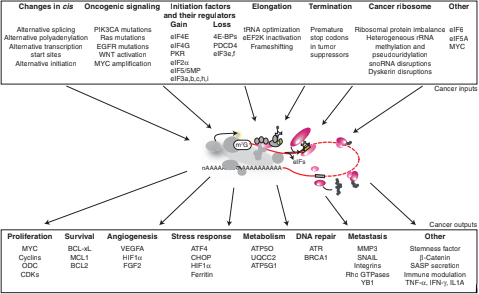
\includegraphics[width=\textwidth]{media/transcontrol.png}
		\end{center}
	\end{frame}
	\begin{frame}
		\frametitle{TransSNP}
		\begin{center}
		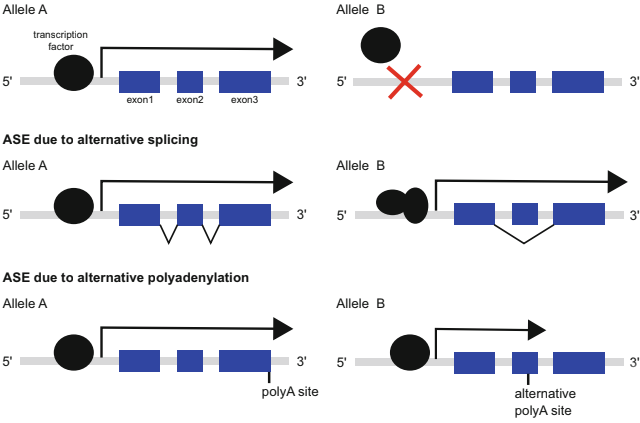
\includegraphics[height=0.8\textheight]{media/snp.png}
		\end{center}
	\end{frame}
	\begin{frame}
		\frametitle{Individuare transSNP}
		\begin{center}
			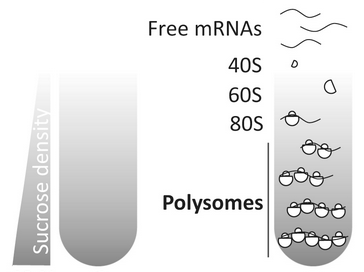
\includegraphics[height=0.8\textheight]{media/polprof.png}
		\end{center}
	\end{frame}
	\begin{frame}
		\frametitle{Campioni}
		\begin{table}
			\begin{tabular}{|c|c|c|}
				\hline
				Nome & Trattamento & Linea cellulare\\
				\hline
				scr\_DMSO & DMSO & HCT116\\
				\hline
				scr\_NUTLIN & NUTLIN & HCT116\\
				\hline
				shDHX30\_DMSO & DMSO & \makecell{HCT116 con knockdown\\di DHX30}\\
				\hline
				shDHX30\_NUTLIN & NUTLIN & \makecell{HCT116 con knockdown\\di DHX30}\\
				\hline
				shPCBP2\_DMSO & DMSO & \makecell{HCT116 con knockdown\\di PCBP2}\\
				\hline
				shPCBP2\_NUTLIN & NUTLIN & \makecell{HCT116 con knockdown\\di PCBP2}\\
				\hline
			\end{tabular}
		\end{table}
	\end{frame}
	\section{Pipeline di analisi}
	\begin{frame}
		\frametitle{Allineamento}
		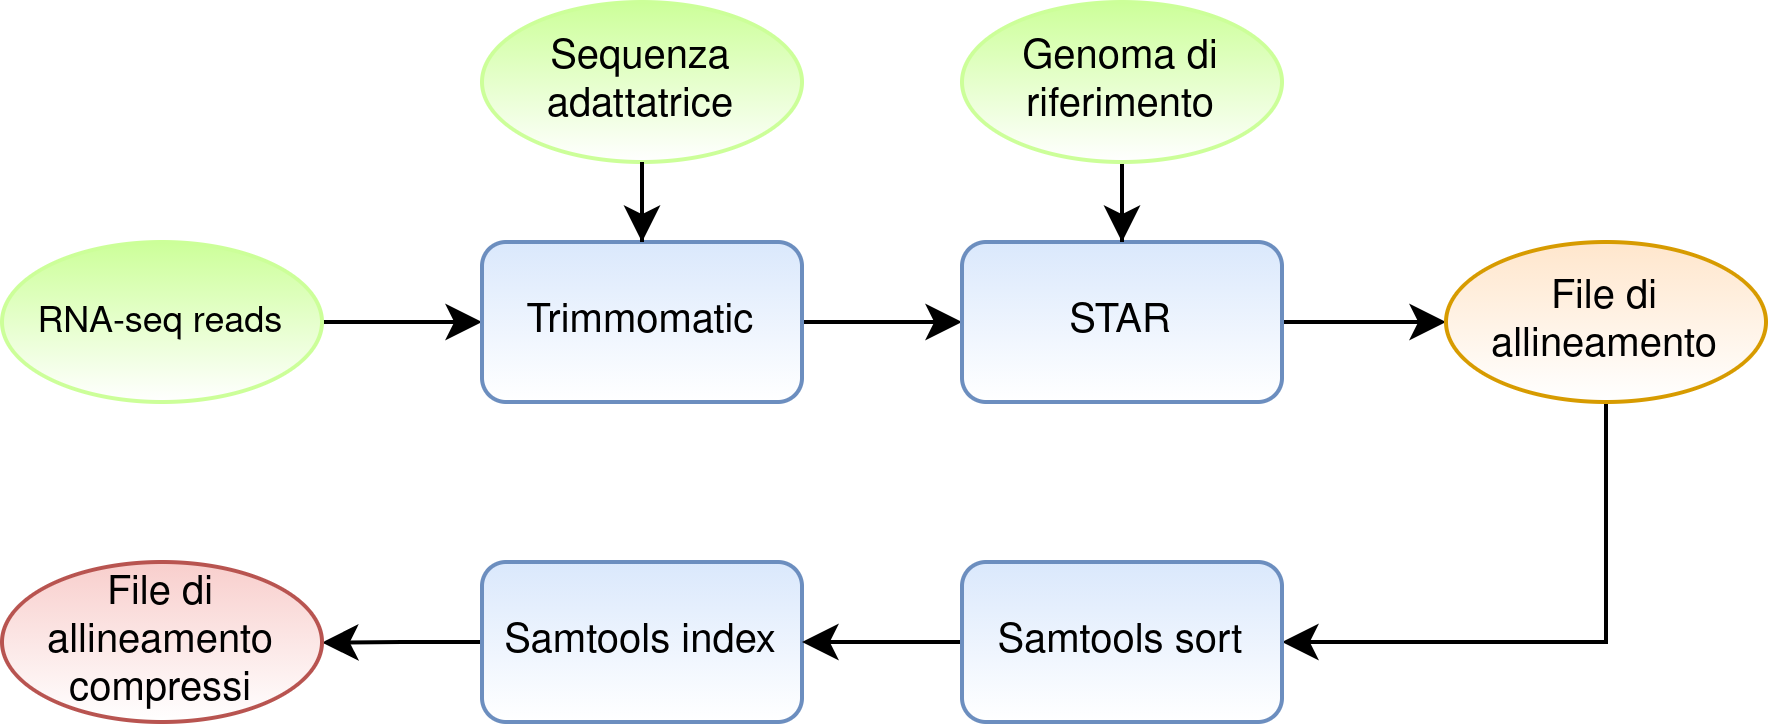
\includegraphics[width=\textwidth]{media/allineamento.png}
	\end{frame}
	\begin{frame}
		\frametitle{Deduplicazione}
		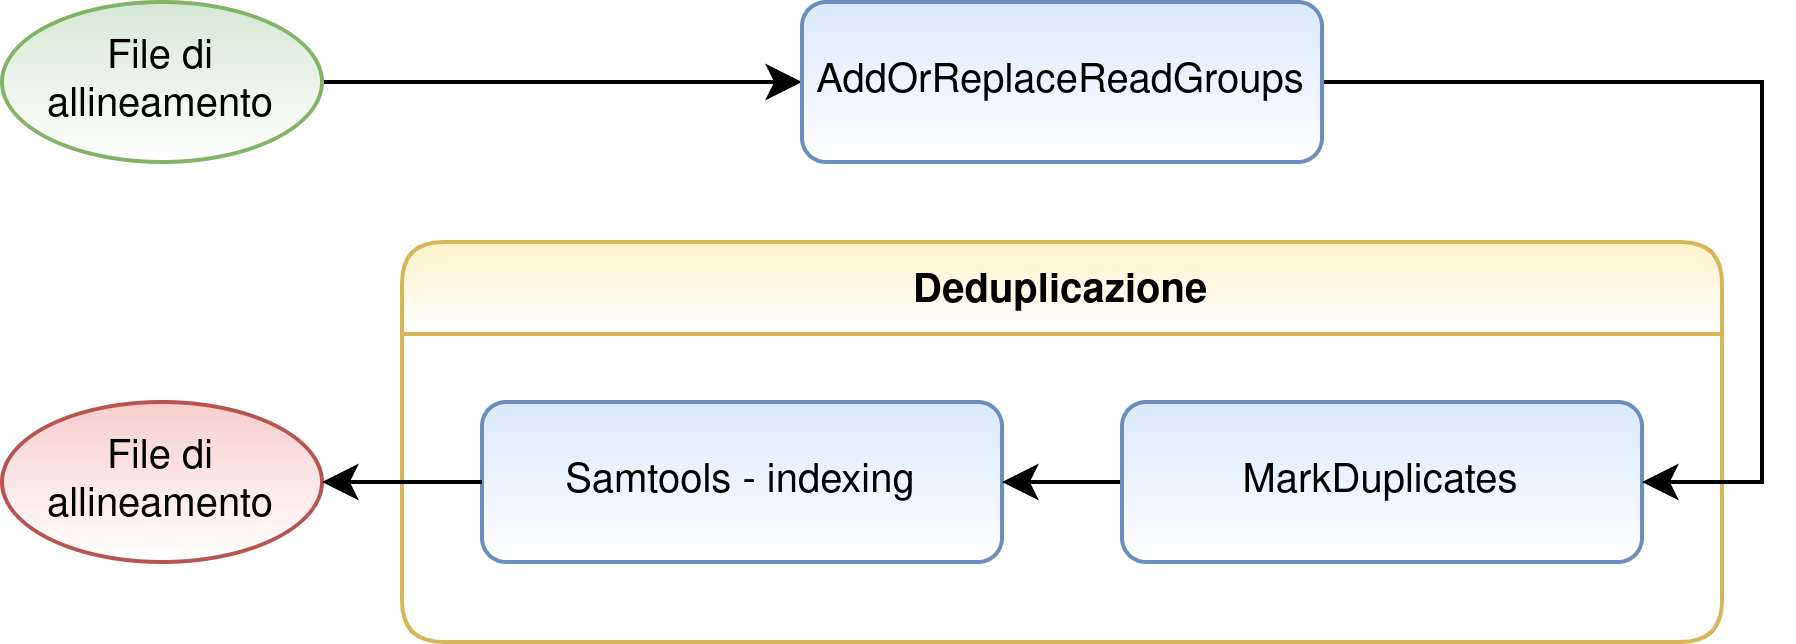
\includegraphics[width=\textwidth]{media/dedup.png}
	\end{frame}
	\begin{frame}
		\frametitle{Riallineamento}
		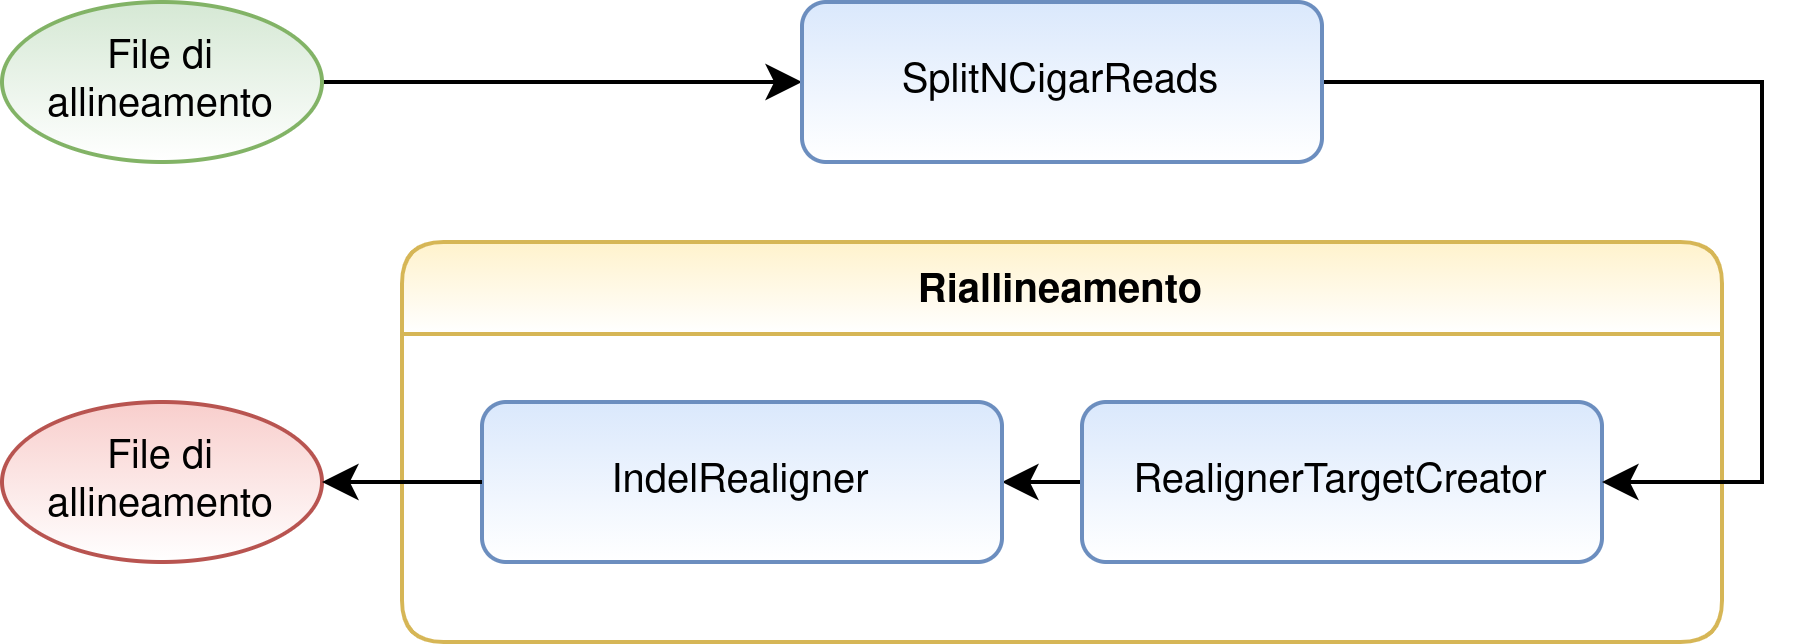
\includegraphics[width=\textwidth]{media/riall.png}
	\end{frame}
	\begin{frame}
		\frametitle{Recalibrazione}
		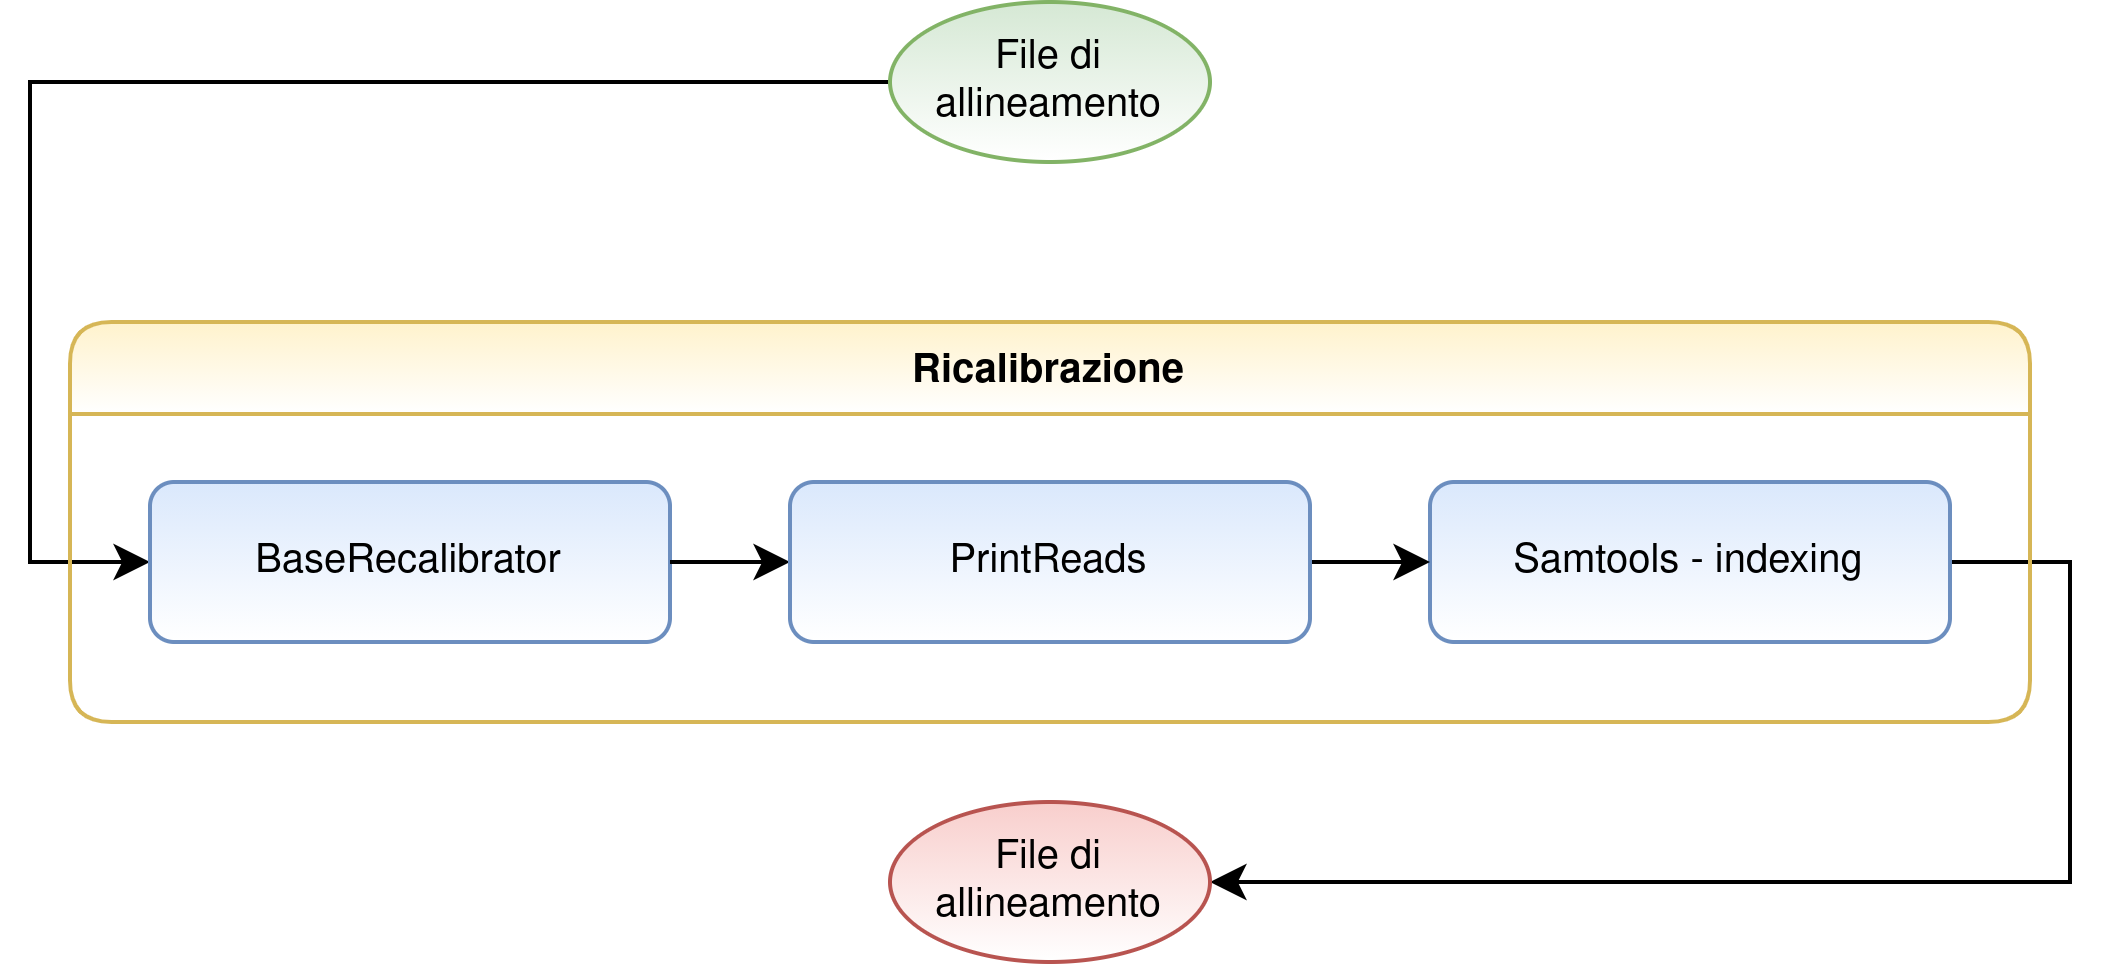
\includegraphics[width=\textwidth]{media/recab.png}
	\end{frame}
	\begin{frame}
		\frametitle{Analisi dati WES}
		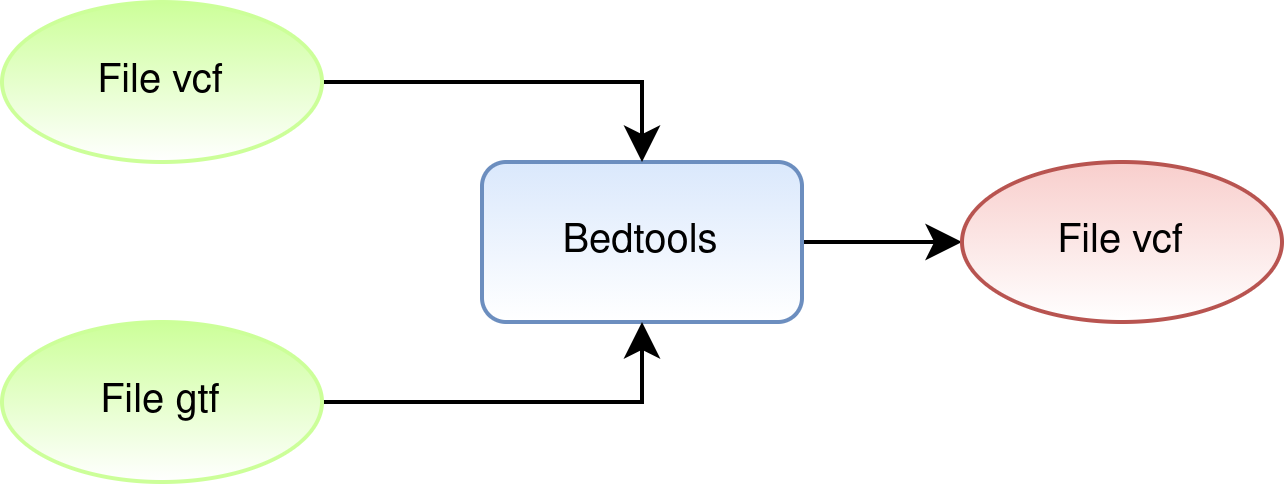
\includegraphics[width=\textwidth]{media/wes.png}
	\end{frame}
	\begin{frame}
		\frametitle{ASEQ}
		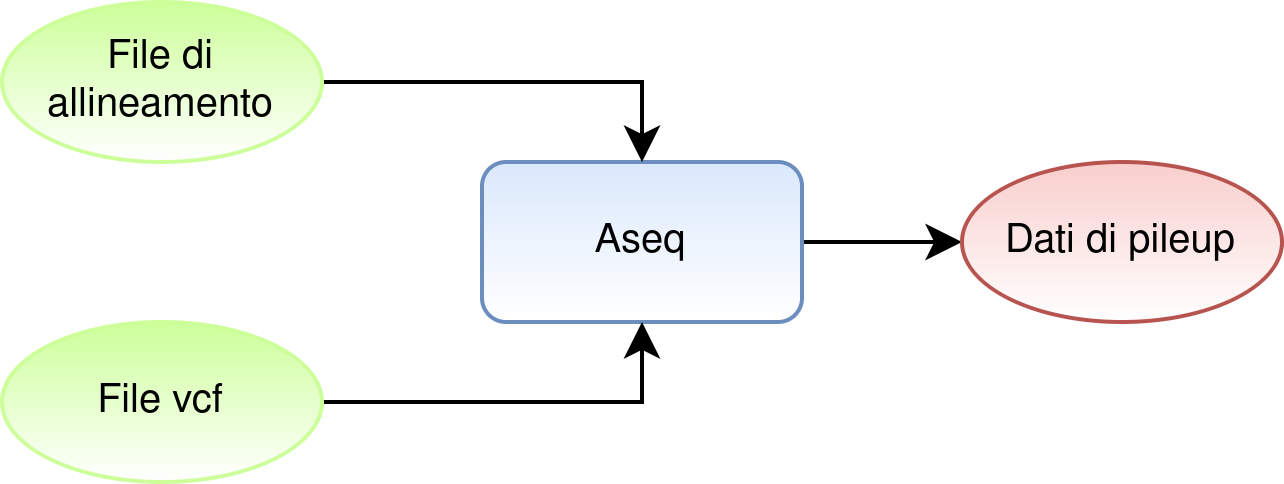
\includegraphics[width=\textwidth]{media/aseq.png}
	\end{frame}
	\section{Risultati ottenuti}
	\begin{frame}
		\frametitle{Analisi dei risultati}
		\begin{table}[H]
			\begin{tabular}{|c|c|c|c|}
				\hline
				Condizione & Totali & $3'$-UTR & $5'$-UTR\\
				\hline
				scr\_DMSO & $27$ & $8$ & $2$\\
				\hline
				scr\_NUTLIN & $33$ & $11$ &$2$\\
				\hline
				shDHX30\_DMSO & $22$ & $9$ & $1$\\
				\hline
				shDHX30\_NUTLIN & $25$ & $11$ & $0$\\
				\hline
				shPCBP2\_DMSO & $24$ & $10$ & $1$\\
				\hline
				shPCBP2\_NUTLIN & $30$ & $11$ & $2$\\
				\hline
			\end{tabular}
			\caption{SNP individuati con p-value nominale inferiore a $0.05$}
		\end{table}
	\end{frame}
	\begin{frame}
			\frametitle{TBC1D9B - scr\_NUTLIN}
		\begin{figure}
			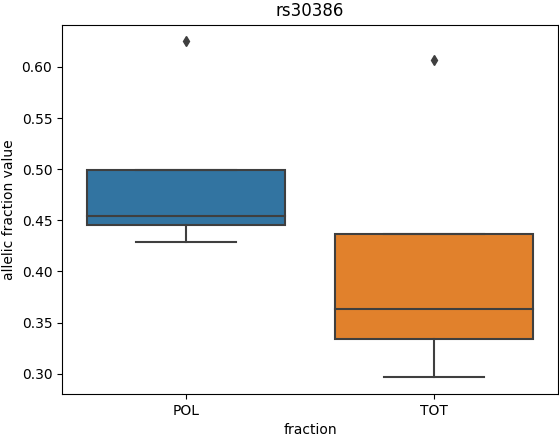
\includegraphics[width=0.84\textwidth]{media/scr_NUTLIN_rs30386.png}
		\end{figure}
	\end{frame}
	\begin{frame}
		\frametitle{SF3B1 - scr\_NUTLIN}
		\begin{figure}
			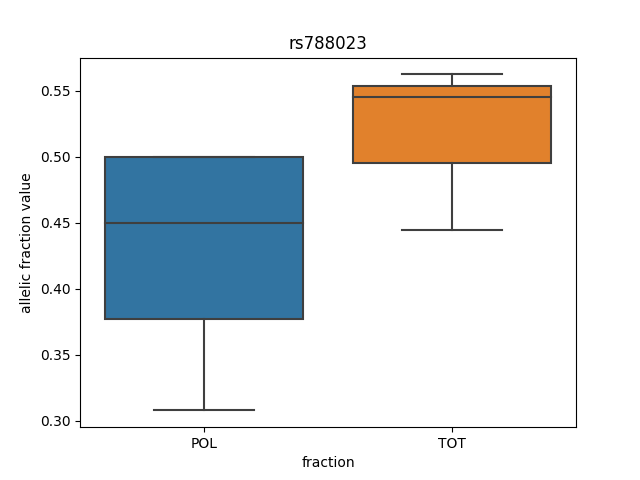
\includegraphics[width=0.84\textwidth]{media/scr_NUTLIN_rs788023.png}
		\end{figure}
	\end{frame}
	\begin{frame}
		\frametitle{KIF5B - shDHX30\_DMSO}
		\begin{figure}
			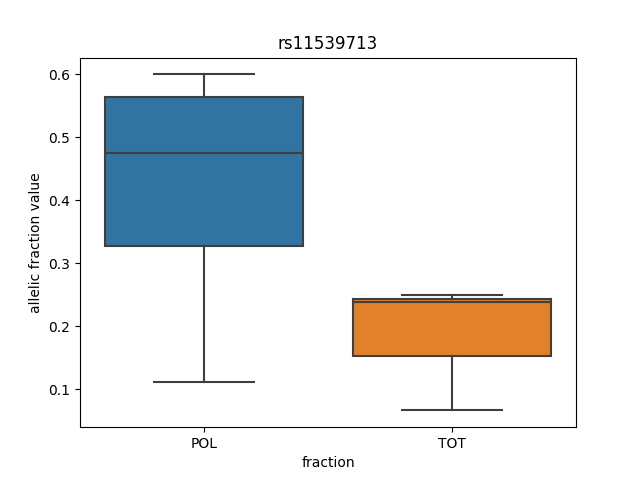
\includegraphics[width=0.84\textwidth]{media/shDHX30_DMSO_rs11539713.png}
		\end{figure}
	\end{frame}

\end{document}
